\documentclass{report}
\usepackage{wallpaper} %Used for the wallpaper
\usepackage{blindtext} % Used for Lorem Ipsum
\usepackage[margin=2cm]{geometry} % Easy way to define margins
\usepackage{fancyhdr} % Fancy header and footer
\pagestyle{fancy}
\usepackage{parskip} % Package to separate paragraphs with a line instead of indentation

\usepackage{multicol} % Needed for three columns (explanation in text).
\usepackage[uppercase]{titlesec} % Used for easy manipulation of section headings.

\usepackage{ifxetex}
\ifxetex
\usepackage{xltxtra} % This package loads fixltx2e, metalogo, xunicode, fontspec
\newfontfamily\ork{Civic}
\setmainfont[Ligatures={Common,TeX}]{Nimbus Sans L}
\else
\usepackage[scaled]{helvet} % Next three lines choose Helvetica as the font.
\renewcommand*\familydefault{\sfdefault} %% Only if the base font of the document is to be sans serif
\usepackage[T1]{fontenc}
\fi

\ifxetex
\titleformat*{\chapter}{\centering\ork\thispagestyle{fancy}}
\else
\titleformat*{\chapter}{\centering\thispagestyle{fancy}}
\fi

\titlespacing\chapter{0pt}{-4ex}{\parskip} % Removing spacing between section headings and their paragraphs
\titlespacing\section{0pt}{0ex}{-\parskip} % Removing spacing between section headings and their paragraphs
\titlespacing\subsection{0pt}{0ex}{-\parskip}
\titlespacing\subsubsection{0pt}{0ex}{-\parskip}

\setcounter{secnumdepth}{-1} % Get rid of all numbering, but let everything turn up in the table of contents

\renewcommand{\headrule}{
\includegraphics[width=180mm]{dirtyheader.png}} % Fancy ork header.

\fancyfoot{} % clearing the footer
\ifxetex
\fancyfoot[LE,RO]{\fbox{\parbox[c]{1.8em}{\ork\centering\vspace{0.5em}\thepage\vspace{0.5em}}}} % put a box around the page number, putting it in the footer. For two-sided documents, it places it (L)eft on (E)ven pages, (R)ight on (O)dd.
\else
\fancyfoot[LE,RO]{\fbox{\parbox[c]{1.8em}{\centering\vspace{0.5em}\thepage\vspace{0.5em}}}} % put a box around the page number, putting it in the footer. For two-sided documents, it places it (L)eft on (E)ven pages, (R)ight on (O)dd.
\fi

%\makeatletter % Anything between this and \makeatother would usually live in a class i.e. commands meant for only a cls file.
%\renewcommand\@maketitle{\centering\Huge\@title\\} % Casually redefining how the title works. NB, this will make twocolumn titles only live in one column.
%\makeatother

\begin{document}
\chapter{WAAAAAAAAAAAAAAAGH!}
%\maketitle
%\thispagestyle{fancy} % Needed to make sure we get the nice header even on the ``titlepage''

\begin{multicols}{3}
\LRCornerWallPaper{1}{background.png}

\section{Caveats}\label{sec:caveats}%
This template was made based on a quick look at an Ork codex.

Other caveats of this template include:
\begin{itemize}
\item No figure environment. There are workarounds, but floats \emph{will not work} in multicol environment. Passing \verb=twocolumn= option to \verb=article= class allows floats (along with the normal \verb=figure*= to span across columns), but then you only have two columns.
\item Footnotes are like this\footnote{See? This footnote will span across the whole page if it gets the chance!}. If you want footnotes that only span the bottom of columns, there are solutions online. Also, footnotes may not appear on the same page as they were referenced. Again, solved by \verb=twocolumn= option used instead.
\item If you want more control of things (e.g.\ having a picture span across only two columns), I recommend the \verb=flowfram= package. It is more complicated that \verb=multicol=, but gives enough control over layout that you could make a professional magazine if you wanted to.
\item Chapter headings probably look best if they are outside the \verb=multicol= environment (this is the default if you use \verb=twocolumn= instead of \verb=multicol=), but you can see for yourself down below.
\end{itemize}

Although there are no figures, you can still create a minipage with an image and some text. Or even just text, for those little stories. In fact, one can probably be very careful and create a \verb=picture= environment with \verb=parbox=s and \verb=includegraphics=s such that you get those nice little text boxes that look like paper.
\fbox{\begin{minipage}[c]{1.0\linewidth}
\LRCornerWallPaper{1}{background.png}
  \vspace{1em}
  \centering
  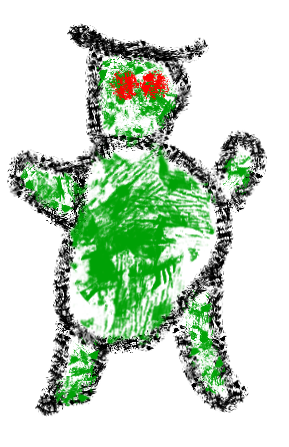
\includegraphics[width=0.7\linewidth]{ork.png}\\
  \it That is one mean looking ork.
  \vspace{1em}
\end{minipage}}

Fancy headings ala 40k codex's are possible through \ifxetex \XeTeX. \else XeTeX. \fi If this document is compiled with \ifxetex \XeLaTeX , \else XeLaTeX, \fi it will try and use the font `Civic' and `Helvetica', so make sure they're installed. If not, Helvetica will be used throughout. The rest of this document is Lorem Ipsum to show how how good it is.

\end{multicols}

\fbox{\begin{minipage}[c]{1.0\linewidth}
  \vspace{1em}
  \centering
  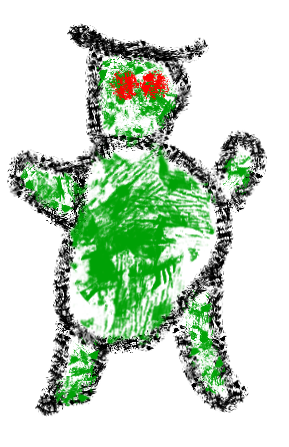
\includegraphics[width=0.3\linewidth]{ork.png}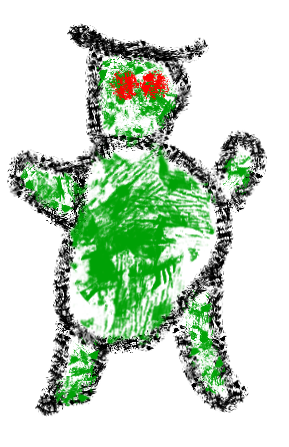
\includegraphics[width=0.3\linewidth]{ork.png}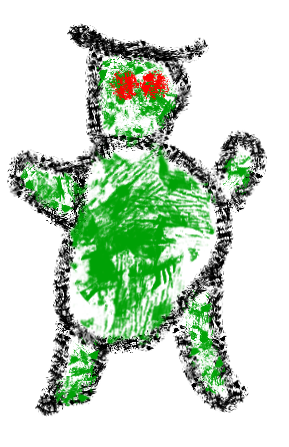
\includegraphics[width=0.3\linewidth]{ork.png}\\
  \it An ork army, spanning the page.
  \vspace{1em}
\end{minipage}}

\begin{multicols}{3}
\blinddocument
\end{multicols}
\end{document}

%%% Local Variables: 
%%% mode: latex
%%% TeX-master: t
%%% End: 
